In this chapter we will outline the project management plan from initiation to delivery. First, an overview over the different parts of the project will be given. Afterwards each phase of the project will be detailed on its own.

\section{Project Outline}
\label{ch:projectplanoutline}

The project is split into five distinct phases shown in figure \ref{fig:projectphases}. The first stage is the initiation phase outlined in \ref{ch:projectinitiation}. It contains the groundwork so the project can go ahead. No specific planning of project work is done in this phase. The second phase contains the planning of the project work and is detailed in \ref{ch:planningphase}. This includes scope management, quality management, project schedule and communications management and is the main part of the project management plan. In the execution phase described in \ref{ch:executionphase} the project work gets carried out. Progress and communications are the key aspects to manage in this phase. The fourth phase is called "Monitoring and Controlling" and describes all actions that need to take place alongside all other phases. This includes, among other things, the validation and control of the scope, quality and schedule defined in the project plan. The last phase detailed in \ref{ch:projectclosing} entails all steps that need to take place in order to deliver the final product, such as demonstration and final presentation.

\begin{figure}
  \centering
  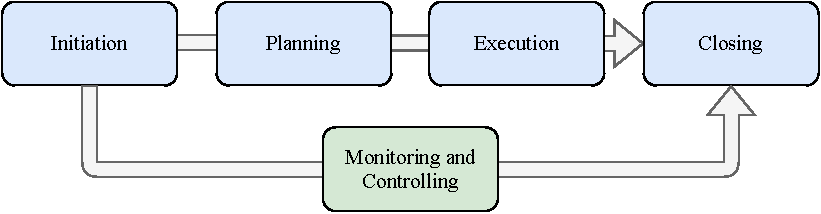
\includegraphics{data/figures/project_lifecycle.pdf}
  \caption{Project Phases}
  \label{fig:projectphases}
\end{figure}


\section{Project Initiation}
\label{ch:projectinitiation}
The project initiation is the first stage of every project. Firstly, the overall goal of the project needs to be defined on a high level. Secondly, the project manager needs to be named. In a project as small as this one, the project manager and the project team are one and the same. Thirdly, the key stakeholders are identified.


\subsection{Project Charter}
\label{ch:projectcharter}
\begin{tcolorbox}
  The overall goal of the project is a well documented implementation of the \ac{AES}. The end result should be a working piece of software that can encrypt and decrypt some input in the way defined in chapter~\ref{ch:aes}.
\end{tcolorbox}


\subsection{Project Team}
\label{ch:projectteam}
In order for the project to start the project team needs to be defined. As this project (the implementation of the \ac{AES}) will be carried out by a team of two, all team decisions have to be made at this stage. At the kick-off meeting for the project teams could be formed. After short private conversation the team for this project was decided. A meeting was setup so the first stages of planning could take place. The team for this project are Jan Phillip Berg and Simon Keil.

\subsection{Stakeholders}
\label{ch:stakeholders}
It is crucial for the project's success to identify the stakeholders and their respective interests, involvement and interdependencies. As this is a project carried out in an academic context, the stakeholders are the lecturers grading and reviewing the final work. They not only have a big impact on project success by grading the end result, but will have an involvement throughout the process with regular feedback. This feedback will be gathered through progress presentations given by the project team every two weeks. As there are no other stakeholders, the project team themselves excluded, there are no interdependencies to manage.


\section{Planning Phase}
\label{ch:planningphase}
The planning phase of the project is where the project management plan is created. This section of the thesis contains the definitions of requirements and scope, as well as the management of schedule, communications, and quality.

\subsection{Scope Management}
\label{ch:scopemanagement}
In most projects the "Magic Triangle" of scope, cost and schedule needs to be managed \cite{vanwyngaard2012}. The academic nature of this project removes considerations for cost, simplifying the planning and giving more room for playing with schedule and scope. The scope of a project should be defined as \textit{all} and \textit{only} the work required to complete the project successfully. We will define the scope of this project in the following sections by first listing the requirements. Afterwards, we will give a scope statement.

\subsubsection{Requirements}
\label{ch:requirements}
The high level goal of the project defined in chapter~\ref{ch:projectcharter} can be extended into some more detailed requirements listed below. The requirements are sorted into the those concerning the software's functionality, the implementation, and the documentation of the software.
\paragraph{Requirements on the software:}
\begin{itemize}
  \item encryption of a text input via AES-128 with a given key
  \item decryption of an encrypted text via AES-128 with a given key
  \item computation of all lookup tables used in AES-128
  \begin{itemize}
    \item computation of the SBox
    \item computation of the Round Constants for the key expansion
  \end{itemize}
\end{itemize}

\paragraph{Requirements on the implementation:}
\begin{itemize}
  \item implementation of \ac{AES} key expansion
  \item separate implementations of en- and decryption
  \item visible and even work-split between team members
  \item steady progress with biweekly presentable results
\end{itemize}

\paragraph{Requirements on the documentation:}
\begin{itemize}
  \item thesis of 20 pages containing:
  \begin{itemize}
    \item theoretical background on symmetric encryption
    \item symmetric encryption use-cases
    \item detailed explanation of the \ac{AES} algorithm
    \item project plan
    \item requirements
    \item deliverables
  \end{itemize}
  \item program documentation of 30 pages containing:
  \begin{itemize}
    \item usage
    \item implementation
    \item functions
    \item performance
    \item software stack
    \item limitations
  \end{itemize}
\end{itemize}

\subsubsection{Scope Statement}
\label{ch:scopestatement}
\begin{tcolorbox}
  The project of implementing the \ac{AES} has to goal of creating a software that can encrypt and decrypt text inputs in AES-128 with a given key. Specifically excluded from the scope are the handling of binary input, AES-256 and up, and the unification of en- and decryption functionality into one callable executable. The software only has run on one common operating system. Further compatibility is excluded from the scope. Documentation of the software and explanations of the \ac{AES}'s functionality are to be included.
\end{tcolorbox}


\subsection{Schedule Management}
\label{ch:schedulemanagement}

In order to develop a schedule the activities must be defined. We will use a work breakdown structure for this purpose, which can be found in section~\ref{ch:wbs}. Afterwards, we will sequence the different work packages and assign them to team members.

\subsubsection{Work Breakdown Structure}
\label{ch:wbs}

The work breakdown structure is shown in figure~\ref{fig:wbs}. It is a hierarchical decomposition of the work that is needed to be done in order to complete the project. The top level of this hierarchy are the five project phases detailed in section~\ref{ch:projectplanoutline}. All components of the \ac{WBS} are numbered. The lowest level component of each branch is a work package that can be scheduled and assigned. The \ac{WBS} does not represent scheduling information. The deliverables of the project can be found in the "Execution" branch.

\begin{figure}
  \makebox[\textwidth]{
  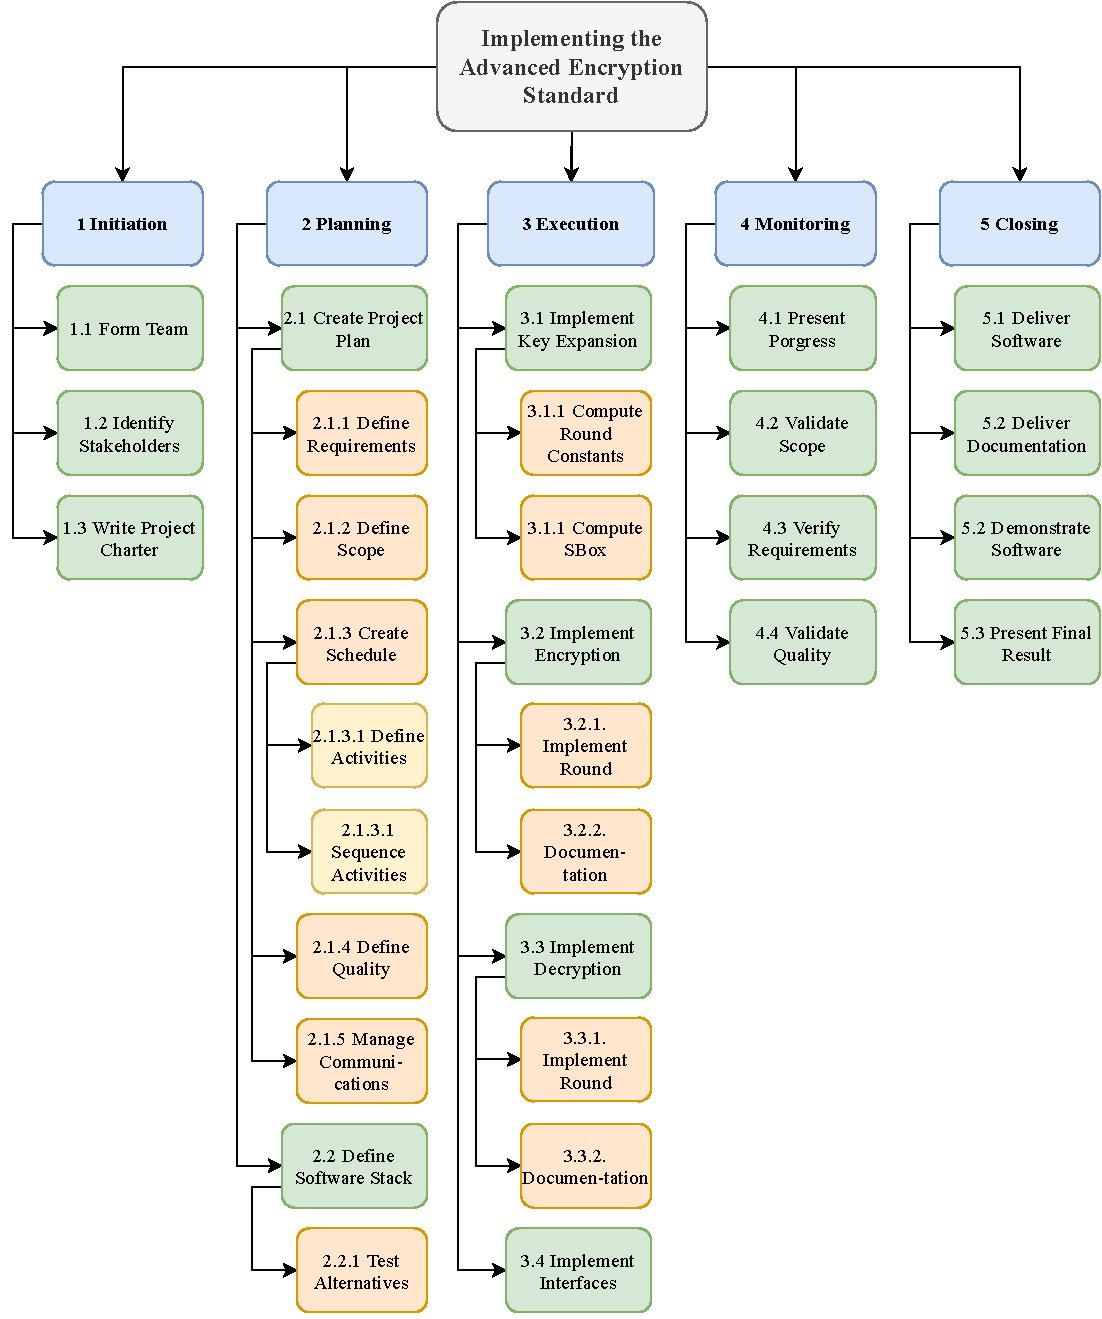
\includegraphics[scale=0.82]{data/figures/WBS.pdf}}
  \caption{Word Breakdown Structure}
  \label{fig:wbs}
\end{figure}


\subsubsection{Sequencing and Assignment of Work Packages}
\label{ch:sequencingandassignment}




\section{Quality Management}
\label{ch:qualitymanagement}
This is a software project and as such we will measure the quality of the work being done in two primary dimensions: Conformity of code to style conventions and performance or efficiency of the program. Conformity to style conventions is important in order to keep the code readable and understandable for third parties. The performance of the program has real world effects for the use of an encryption program. If the runtime is too long, encrypting large files becomes impractical.

\subsection{Code Quality}
\label{ch:codequality}
For Python code we will refer to the PEP-8 style guide \cite{pep8}. Code files will be organized by logical program parts. For C Code we will refer to the .... style guide. We will include C source files as well as header files in the code directories. Functions should have docstrings. Where inline comments are necessary to explain actions, their use is encouraged. In general, the use of inline comments should be minimal.

\subsection{Program performance}
\label{ch:programperformance}
Program performance highly depends on the time complexity of the algorithms, the inputs to the program, as well as the software stack that is used. As the algorithm and the inputs are given for this project, the software stack is the major contributing factor to program performance. In general, the lower level a language is, the faster you can make a program. Writing the software in assembly or even a hardware description language to program a \ac{FPGA} would yield the best results. However, we deem these options to be out of scope for this project. Which software stack was chosen and why is detailed in section~\ref{ch:softwarestack}.

To measure the performance of our implementation, reference implementations in various higher level languages are given the same inputs. We then compare the results with our solution. For the different subparts of the program, different implementations of single functions are to be tested against each other to find the best compromise between performance and code quality. An example of this would be converting string inputs into bytes through string operations versus through bit-shifts.

The quality goal for performance is an implementation that is faster than implementations in pure Python.

DIFFERENT TIMINGS HERE

\subsection{Software Stack}
\label{ch:softwarestack}
The selection of the software stack depends on a few major factors. Those factors are the platform the program should run on, developer experience, and performance. The stack that was chosen for this project is shown in figure~\ref{fig:stack}

In the team formation process discussed in section~\ref{ch:projectteam} the literacy in various programming languages was a key component. We decided on Python 3 as our wrapper language. This means all one-time operations will be written in Python. This makes the code readable without incurring major performance penalties. Another advantage of using Python is that the software will run on most platforms. Both team members are fluent and have experience writing code in Python.

The performance goals defined in section~\ref{ch:programperformance} are not reachable with pure Python. Therefore, we select to write the core algorithms in C. The main benefit of this hybrid approach is performance. The disadvantage is the increased code complexity inherent to C. The approach also requires an interface between C and Python.

After testing different interface solutions we settled on the ctypes module for Python 3 \cite{ctypes}. The major advantage is that we can write normal independent C code and compile it separately. Other solutions would have required non-standard interpreters or compilers (see Cython \cite{cython}). The interface works by compiling the C code into libraries and importing those into a Python program. The functions within are then callable in Python. Intercompatibility between platforms is maintained by shipping with C source and header files. Compilation can be done according to the platform.

\begin{figure}
  \centering
  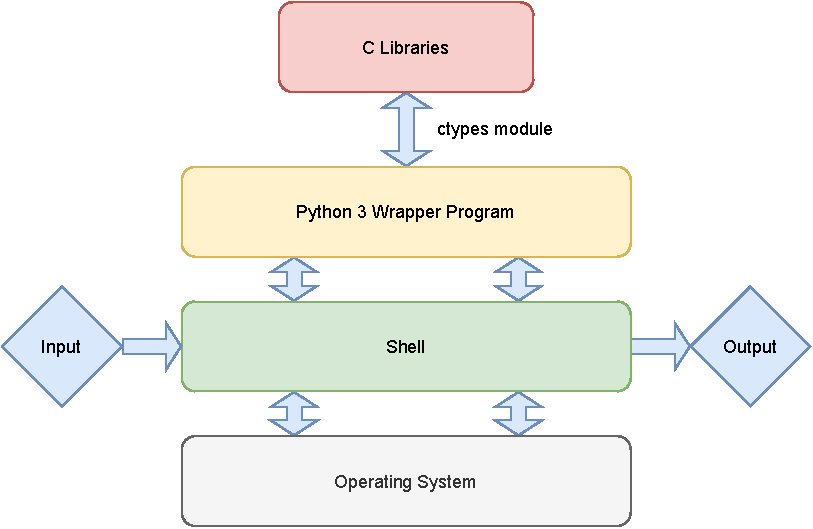
\includegraphics{data/figures/stack.pdf}
  \caption{Software Stack}
  \label{fig:projectphases}
\end{figure}


\subsection{Communications Management}
\label{ch:communicationsmanagement}
Communication is a key part of every project. Even though the team for this project only has two members communication channels need to be well defined. In software project such as this one the source code management is also a concern. Another key component of the communications management is the engagement with the projects stakeholders. The communication channels for all these purposes are detailed below.

\subsubsection{Source Code Management and Version Control}
\label{ch:versioncontrol}
The version control tool of choice is Git \cite{git}. A remote repository will be hosted on \url{github.com}. We follow a loose feature-branch workflow. Separate branches are created for the key components (work packages 3.1, 3.2, 3.4 see~\ref{ch:wbs}) of the software, as well as for the documentation and thesis documents. Team members work on the branches of the work packages they are assigned to (see ~\ref{ch:sequencingandassignment}). Merging into other branches occurs when the component is complete. Testing is done on each component separately before merging.


\subsubsection{Day to Day Communications}
\label{ch:daytodaycomms}
For day to day issues a WhatsApp chat is used as the primary communications channel. It ensures high availability. Reasons to use this channel might be: arranging of code interfaces, scheduling of meetings, and questions or problems regarding project. Progress is discussed in regular meetings via Zoom. These meetings are scheduled at least weekly.


\subsubsection{Stakeholder Engagement}
\label{ch:stakeholerengagement}
As discussed in section~\ref{ch:stakeholders}, the main stakeholders for this project are the lecturers grading the final work. They are engaged in the process through biweekly presentations of the progress. These presentations are around ten minutes in length and entail both team members discussing their progress during the time in between sessions. Both team members need to present their respective work and demonstrate the even split of workload during the whole project. Stakeholder engagement is important in order to keep on track and avoid scope- or schedule creep.


\section{Execution Phase}
\label{ch:executionphase}
The execution phase is the main part of the project. The team members work on their assigned \ac{Wp}s and create the deliverables for the project. All parts of the project done in this phase can be found in execution branch of the \ac{WBS}. While implementation and documentation takes place, the communication needs to be managed according to the communications management plan laid out in section~\ref{ch:communicationsmanagement}. Regular meetings between team members take place to discuss progress and problems that might have arisen. Progress presentations to the stakeholders happen biweekly. In addition to the main tasks, these presentations need to be prepared. This is an important step in order for the team to mark the progress.

While the main \ac{WP}s get worked on, the monitoring and controlling processes detailed in section~\ref{ch:monitoringcontrolling} need to be carried out alongside. This mainly includes the testing of implemented functionality. Rigorous testing and validation ensures the final software is inside the defined quality and scope. Readjustments to scope and requirements need to be made whenever there is new input from the stakeholders or the current scope or requirements are not achievable any more. Regular reassessment and verification is crucial to project success.


\section{Monitoring and Controlling}
\label{ch:monitoringcontrolling}
This section details the processes that take place alongside the main schedule. They serve the purpose to keep the project on track, meaning in scope, in quality, and on schedule. Without these processes project success is much harder to achieve. As these monitoring and controlling functions are regular tasks each team member needs to do they are listed in the \ac{WBS}. In the following, these processes are described in further detail.

\subsection{Validate Scope}
\label{ch:validatescope}
Every time a \ac{WP} is completed, the project team will validate that the deliverable is inside project scope. If it is not sufficient, a change request will be made to the assigned team member. They will start implementing the changes decided on. This workflow ensures all deliverables meet the requirements and that the project is in scope.

In regular intervals the project team will reassess whether the scope statement (see section~\ref{ch:scopestatement}) is still accurate. The project scope will be adjusted if stakeholders demand changes or if the schedule cannot be met. Such changes need to be decided on with the whole project team. They need to be formalized in a new scope statement and changes to the \ac{WBS} and schedule need to be made accordingly. This formalization of changes is important to ensure all team members are on the same page regarding the scope of the project.

\subsection{Verify Requirements}
\label{ch:verifyrequirements}
In accordance with the workflow laid out in section~\ref{ch:validatescope}, finished \ac{WP}s need to be assessed against the project requirements. If the deliverable is lacking, change requests are implemented. Alongside the verification of requirements for each \ac{WP}, the project requirements need to be reevaluated analogous to scope reassessment. New requirements can only be added if formalized. Sources of changes to the requirements are schedule conflicts and stakeholder requests.

\subsection{Validate Quality}
\label{ch:validatequality}
Each function in the program code needs to be validated on its quality. The guidelines for quality can be found in section~\ref{ch:qualitymanagement}. In regular progress meetings the team members talk each other through all \ac{WP}s they are working on (finish as well as in progress). Assessments regarding code quality and conformity to style conventions can be made in these meetings. Checking for style conventions will also be automated in the Git repository.

Each team member is responsible for testing their code throughout the process. Bugs are to be fixed in order to maintain a working program. When user input is taken, it needs to be properly escaped. Testing for edge-cases needs to be done. Testing for program performance will at the delivery of each larger component (\ac{WP} 3.1, 3.2, 3.3, 3.4). If performance is lacking, the team member assigned to that component needs to optimize the code. Solutions for optimization problems can be found in weekly meetings.

\subsection{Present Progress}
\label{ch:presentprogress}
As detailed in section~\ref{ch:stakeholerengagement}, biweekly progress presentations will take place during the project duration. In these presentations each project team member will present what they have accomplished over the last two weeks. This monitoring process is important in order to keep the work going at a steady rate and ensure an equal work split between team members. These presentations are as much for the stakeholders as they are for the project team. The regularity of presentations keeps the team schedule by having external deadlines.


\section{Project Closing and Delivery}
\label{ch:projectclosing}
When all project work is done, all deliverables will be combined into one release. The release will contain the final software as defined by the scope statement in section~\ref{ch:scopestatement}. Alongside the software the final delivery will include the thesis and program documentation as mentioned in section~\ref{ch:requirements}. Before delivering, the project team will run through the monitoring processes again to ensure the final delivery is in scope and up to the defined quality standards. The last progress presentations will be a demonstration of the final software as well as short presentation of all its source code. This presentation constitutes the delivery of the final product.

After the conclusion of the project, a reflection phase might occur. The team will meet to discuss what did and what did not go to plan in order to learn from shortcomings.




% \bibliography{references.bib} needed to fix autocompletion for citation in my editor
